\section{Key-value server}
During the first four milestones, we were tasked with developing a distributed key-value storage system, which includes many features such as replication and caching. In this section, we focus on the implementation behind some of those properties.

\begin{figure}[h]
	\centering
	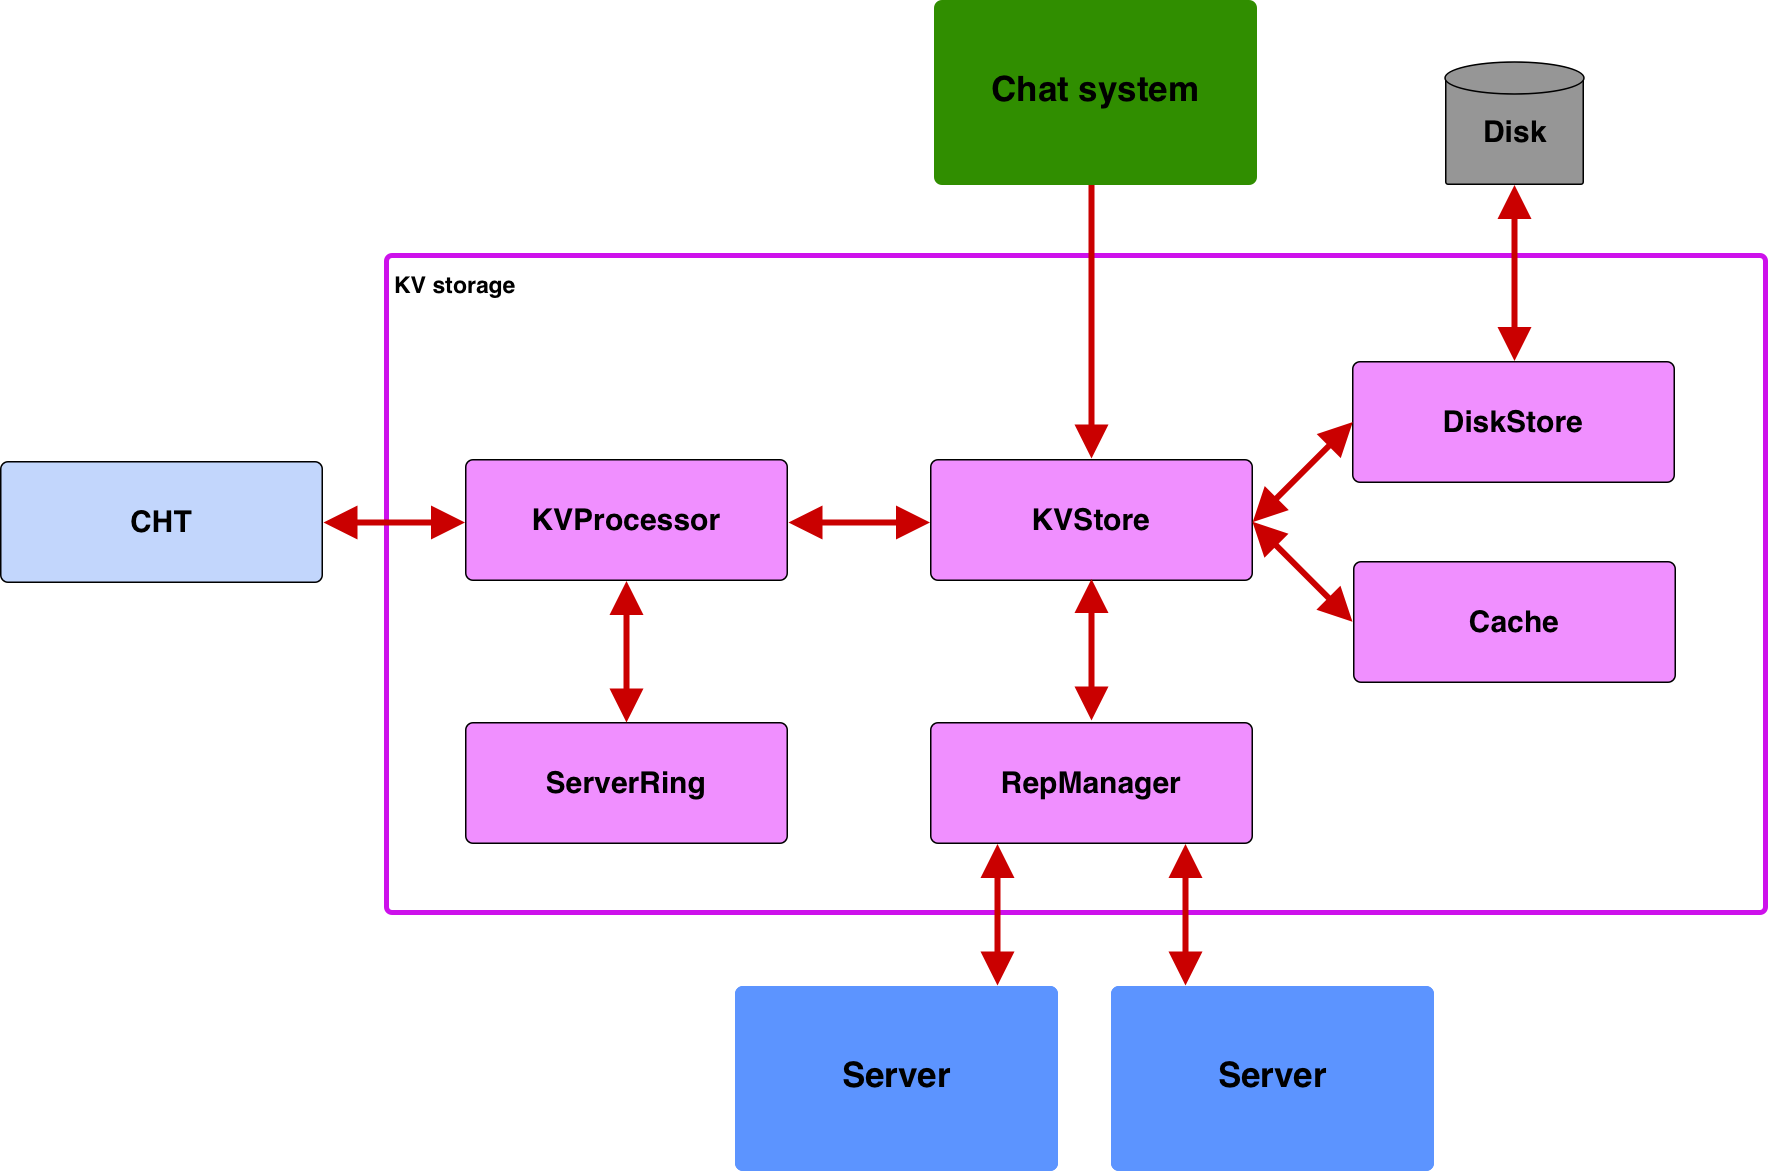
\includegraphics[width=\linewidth]{figures/kvs_arch.png}
	\caption{Client side architecture}
\end{figure}

\subsection{Key-value store}
Key-value stores are perhaps the simplest type of a NoSQL database. Values, which in our case are limited to strings, can be easily stored and retrieved just by providing the key they were assigned with. 

\subsection{Persistence}
%TODO add how data gets stored on disk

\subsection{Caching}



